\section{Delsystem}

Systemet är indelat i två olika delsystem. Dessa system kommer köras
sekvensiellt, alltså det ena efter det andra. Det första systemet kontrollerar
själva bilkörningen medan det andra systemet kontrollerar displayen. Se
figur~\ref{fig:system_diagram} för ett processchema.

\begin{figure}
  \centering
  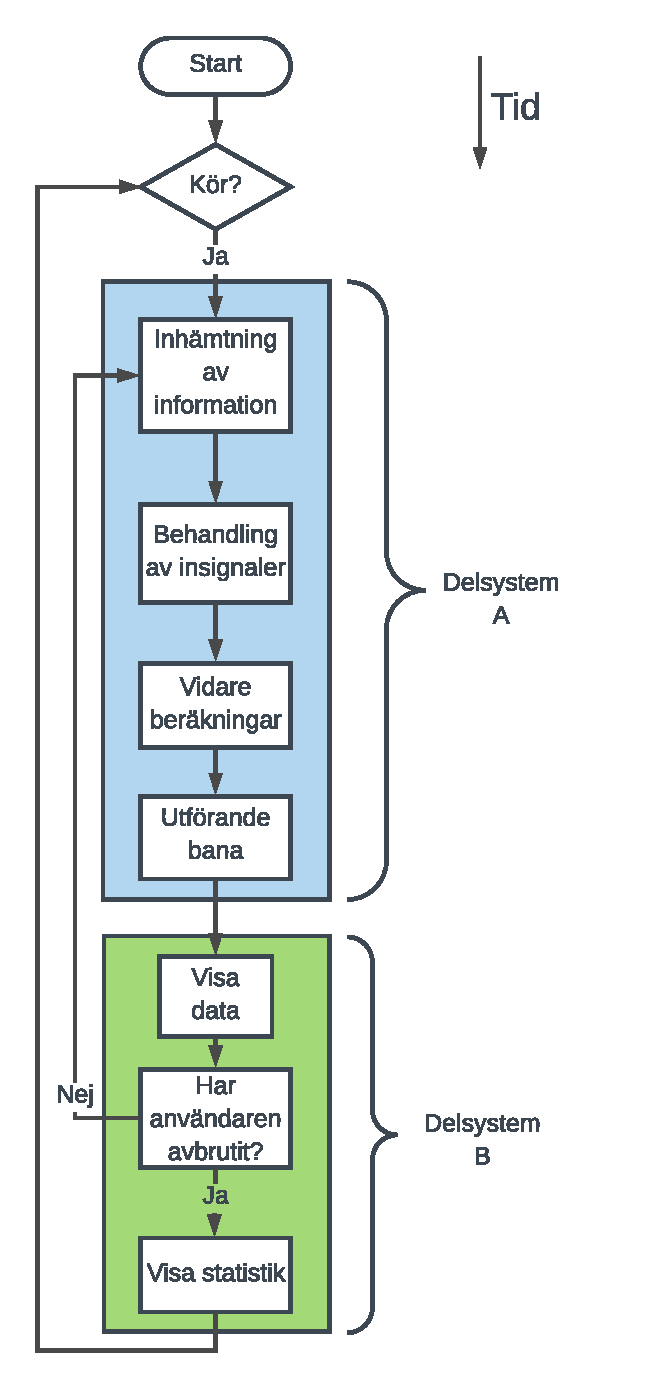
\includegraphics{figures/Processchema.pdf}
  \caption{Processchema över systemets helhet.}
  \label{fig:system_diagram}
\end{figure}

  \subsection{Delsystem A: Bana}
  
  Delsystem A är indelat i tre övergripande delar. I del A.1 hämtas all
  tillgänglig information in, i del A.2a görs beräkningar utifrån tillgänglig
  data, i del A.2b görs vidare beräkningar (alltså beräkningar som inte baseras
  direkt på den tillgängliga informationen), och i del A.3 utförs de ändringar
  som programmet bedömer är nödvändiga för att klara den valda varvtiden. 

    \subsubsection{Inhämtning av information}

    Information som finns tillgänglig är kraftigt begränsad. I praktiken kommer
    programmet endast fråga om någon av bilarna passerat en givare sedan
    programmet frågade förra gången.

    \subsubsection{Primära beräkningar}

    De primära beräkningarna är de beräkningar som beror direkt på tillgänglig
    information. Eftersom indatan enbart består av bilens position är bilens
    hastighet genom det förra segmentet den enda informationen som direkt beror
    på indata.

    \subsubsection{Sekundära beräkningar}
    
    Den första beräkningen som görs är bilens nuvarande position. Detta görs med
    hjälp av en intern bild av banan och vetskapen om vilken hastighet bilen
    önskas ha. Sedan räknas den position som bäst gör att bilen klarar den satta
    varvtiden ut. För att räkna ut den beaktas enbart den nuvarande tiden och
    (om gemensam målgång är aktiverat) positionen av den andra bilen. Steget
    efter är att räkna ut den mest rimliga optimala situationen som beaktar hur
    lång tid det är kvar på det nuvarande varvet. I början av varvet görs alltså
    inte lika drastiska hastighetsändringar som mot slutet.

    Det sista som händer är när informationen om bilens och banans skick används
    för att räkna ut vilket spänningspådrag som krävs för att få bilen att nå
    den hastighet och position som krävs.

    \subsubsection{Utförande}

    I utförandet skickas det nya spänningspådraget till banorna.

  \subsection{Delsystem B: Display}

  Displayen ter sig enklare än delsystem A. Under körning ska, om ett nytt varv
  påbörjats, den senaste varvtiden och varvnumret skickas till displayen. Om
  stopp-knappen har tryckts ned ska systemet hoppa till resultat-skärmen och om
  inte så ska det fortsätta.

  \textbf{Utöver det här ska vi införa en mer detaljerad funktionell beskrivning
  av de olika delsystemen.}
